\documentclass[12pt, spanish]{article}
\usepackage[spanish]{babel}
\selectlanguage{spanish}
%\usepackage{natbib}
\usepackage{url}
\usepackage[utf8x]{inputenc}
\usepackage{graphicx}
\graphicspath{{images/}}
\usepackage{parskip}
\usepackage{fancyhdr}
\usepackage{vmargin}

\usepackage{minted}
\usemintedstyle{vim}

\usepackage{hyperref}
\usepackage[
    type={CC},
    modifier={by-nc-sa},
    version={4.0},
]{doclicense}

\hypersetup{
    colorlinks=true,
    linkcolor=blue,
    filecolor=magenta,      
    urlcolor=cyan,
}

\usepackage[default]{sourcesanspro}

\usepackage[nottoc]{tocbibind}

\setmarginsrb{2 cm}{1 cm}{2 cm}{2 cm}{1 cm}{1.5 cm}{1 cm}{1.5 cm}

\title{Ingeniería de Servidores:\\
Phoronix Test Suite. \hspace{0.05cm} }                           
\author{Antonio David Villegas Yeguas}                             
\date{\today}                                           

\renewcommand*\contentsname{hola}

\makeatletter
\let\thetitle\@title
\let\theauthor\@author
\let\thedate\@date
\makeatother

\pagestyle{fancy}
\fancyhf{}
\rhead{\theauthor}
\lhead{\thetitle}
\cfoot{\thepage}

\begin{document}
%%%%%%%%%%%%%%%%%%%%%%%%%%%%%%%%%%%%%%%%%%%%%%%%%%%%%%%%%%%%%%%%%%%%%%%%%%%%%%%%%%%%%%%%%

\begin{titlepage}
    \centering
    \vspace*{0.5 cm}
    
\includegraphics[scale = 0.50]{ugr.png}\\[1.0 cm]
    %\textsc{\LARGE Universidad de Granada}\\[2.0 cm]   
    \textsc{\large 3ºA - A2}\\[0.5 cm]            
    \textsc{\large Grado en Ingeniería Informática}\\[0.5 cm]              
    \rule{\linewidth}{0.2 mm} \\[0.2 cm]
    { \huge \bfseries \thetitle}\\
    \rule{\linewidth}{0.2 mm} \\[1 cm]
    
    \begin{minipage}{0.4\textwidth}
        \begin{flushleft} \large
            \emph{Autor:}\\
            \theauthor
            \end{flushleft}
            \end{minipage}~
            \begin{minipage}{0.4\textwidth}
            \begin{flushright} \large
            \emph{Asignatura: \\
            Ingeniería de Servidores}                   
        \end{flushright}
    \end{minipage}\\[0.5cm]
  
    {\large \thedate}\\[0.5cm]
    {\url{https://github.com/advy99/ISE/}}
    {\doclicenseThis}
 	
    \vfill
    
\end{titlepage}

%%%%%%%%%%%%%%%%%%%%%%%%%%%%%%%%%%%%%%%%%%%%%%%%%%%%%%%%%%%%%%%%%%%%%%%%%%%%%%%%%%%%%%%%%

\tableofcontents
\pagebreak

%%%%%%%%%%%%%%%%%%%%%%%%%%%%%%%%%%%%%%%%%%%%%%%%%%%%%%%%%%%%%%%%%%%%%%%%%%%%%%%%%%%%%%%%%


\section{Phoronix Test Suite}

Phoronix Test Suite\cite{pts} es un software que nos permite ejecutar un conjunto de benchmarks, ya sean benchmarks propios o usando la plataforma OpenBenchmarking\cite{obm}.

En esta práctica vamos a ejecutar distintos benchmarks sobre el anfitrión, la máquina virtual de Ubuntu Server y la máquina virtual de CentOS.

Antes de realizar los test, debido a la configuración de los distintos sistemas sabemos que el que mejor rendimiento obtendrá será el anfitrión, ya que este puede acceder a la totalidad de los recursos (en mi caso 8 núcleos de un Intel i5-8250U y 8 GB de memoria RAM DDR4) mientras que las máquinas virtuales solo a parte de esta (1 núcleo del Intel i5-8250U y 1 GB de RAM DDR4).

\subsection{Instalación de Phoronix Test Suite}

Para la instalación de Phoronix Test Suite el guión de prácticas nos recomendaba instalarlo desde el gestor de paquetes de los distintos sistemas operativos usados, sin embargo, debido a que las versiones están bastante desactualizadas y ara usar Phoromatic necesitaremos una versión superior a la 9.0.0, lo instalará de forma manual.

\subsubsection{Instalación en el anfitrión (ArchLinux)}

En mi caso, el anfitrión tiene instalado como sistema operativo ArchLinux. A pesar de que la instalación de forma manual es muy sencilla, este sistema operativo cuenta con un script creado por la comunidad para instalarlo. Nos bastara con instalar el paquete comunitario phoronix-test-suite desde el AUR.

En mi caso, al usar YAY\cite{yay} como AUR Helper basta con la siguiente orden en bash:

\begin{minted}[linenos,tabsize=2,breaklines]{bash}
\$ yay -S phoronix-test-suite 
\end{minted}


\subsubsection{Instalación en Ubuntu Server}

Para instalar Phoronix Test Suite basta con descargar el paquete disponible para cualquier distribución en la página de descargas de Phoronix\cite{pts_descarga}, extraer el paquete y ejecutar el script de instalación:

\begin{minted}[linenos,tabsize=2,breaklines]{bash}
\$ wget  https://phoronix-test-suite.com/releases/phoronix-test-suite-9.2.0.tar.gz
\$ tar -xvf phoronix-test-suite-9.2.0.tar.gz
\$ cd phoronix-test-suite/
\$ sudo ./install-sh
\end{minted}

Además tendremos que instalar algunos paquetes de PHP:

\begin{minted}[linenos,tabsize=2,breaklines]{bash}
\$ sudo apt install php-xml php-gd
\end{minted}

Y con esto tendremos instalado Phoronix Test Suite en nuestro Ubuntu Server.

\begin{center}
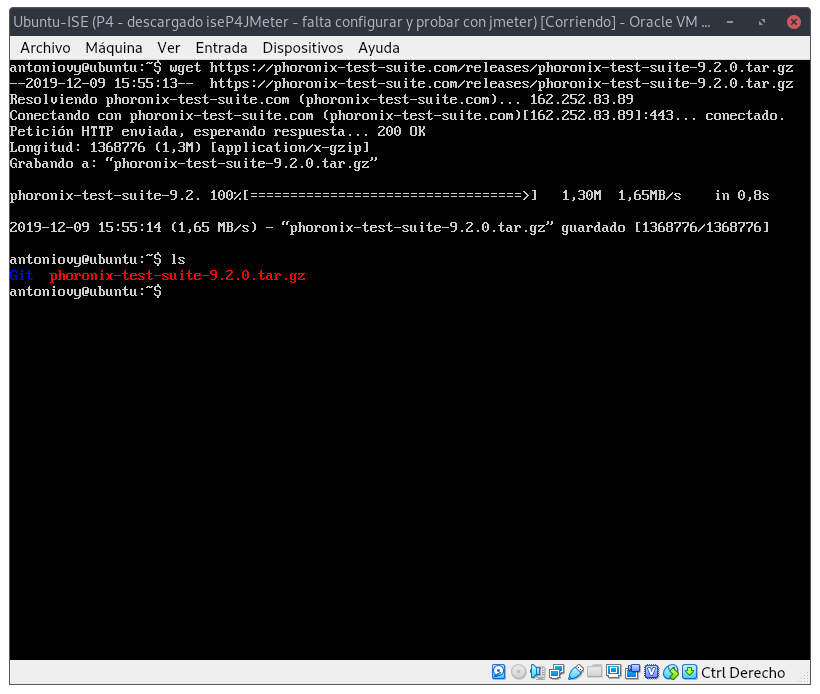
\includegraphics[scale=0.35]{descarga_pts.png}
\end{center}

\begin{center}
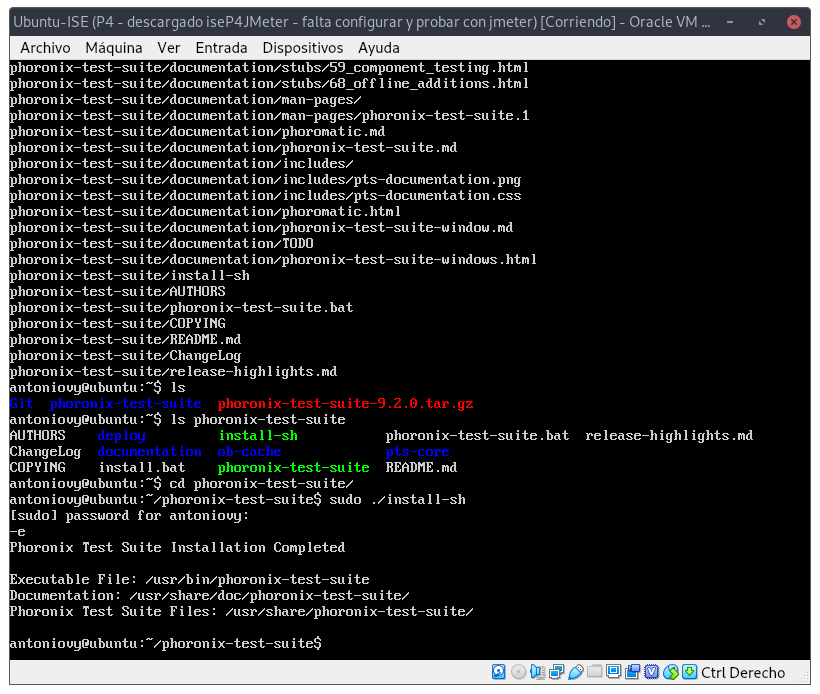
\includegraphics[scale=0.35]{instalacion_pts.png}
\end{center}


\subsection{Instalación en CentOS}

Al igual que con Ubuntu, descargamos el paquete y ejecutamos el script de instalación:

\begin{minted}[linenos,tabsize=2,breaklines]{bash}
\$ wget  https://phoronix-test-suite.com/releases/phoronix-test-suite-9.2.0.tar.gz
\$ tar -xvf phoronix-test-suite-9.2.0.tar.gz
\$ cd phoronix-test-suite/
\$ sudo ./install-sh
\end{minted}


\subsection{Instalación con Docker}

Otra opción es instalar Phoronix Test Suite a través de Docker\cite{pts_docker}

\begin{minted}[linenos,tabsize=2,breaklines]{bash}
\$ docker pull phoronix/pts
\end{minted}

Y ejecutarlo con:

\begin{minted}[linenos,tabsize=2,breaklines]{bash}
\$ docker run -it phoronix/pts
\end{minted}



\subsection{Ejecución de pruebas}

Una vez instalado, podremos realizar pruebas con la siguiente orden:

\begin{minted}[linenos,tabsize=2,breaklines]{bash}
\$ phoronix-test-suite benchmark <nombre_prueba>
\end{minted}

Algunas de las pruebas que he realizado y veremos más adelante son apache (benchmark que utiliza AB), php y smallpt (pequeña prueba para el procesador)


\subsection{Configuración de Phoromatic}

En mi caso ejecutaré el servidor de Phoromatic desde mi anfitrión con la ayuda del manual de phoronix-test-suite\cite{pts_man}.

Para configurar Phoromatic debemos incluir algunas extensiones de PHP, editando el archivo /etc/php/php.ini

\begin{minted}[linenos,tabsize=2,breaklines]{bash}
\$ sudo vim /etc/php/php.ini
\end{minted}

Y descomentamos las extensiones \texttt{sockets}, \texttt{sqlite3} y \texttt{zip}.


Con esto podemos pasar a ejecutar el servidor de Phoromatic con la siguiente orden:

\begin{minted}[linenos,tabsize=2,breaklines]{bash}
\$ phoronix-test-suite start-phoromatic-server
\end{minted}


\begin{center}
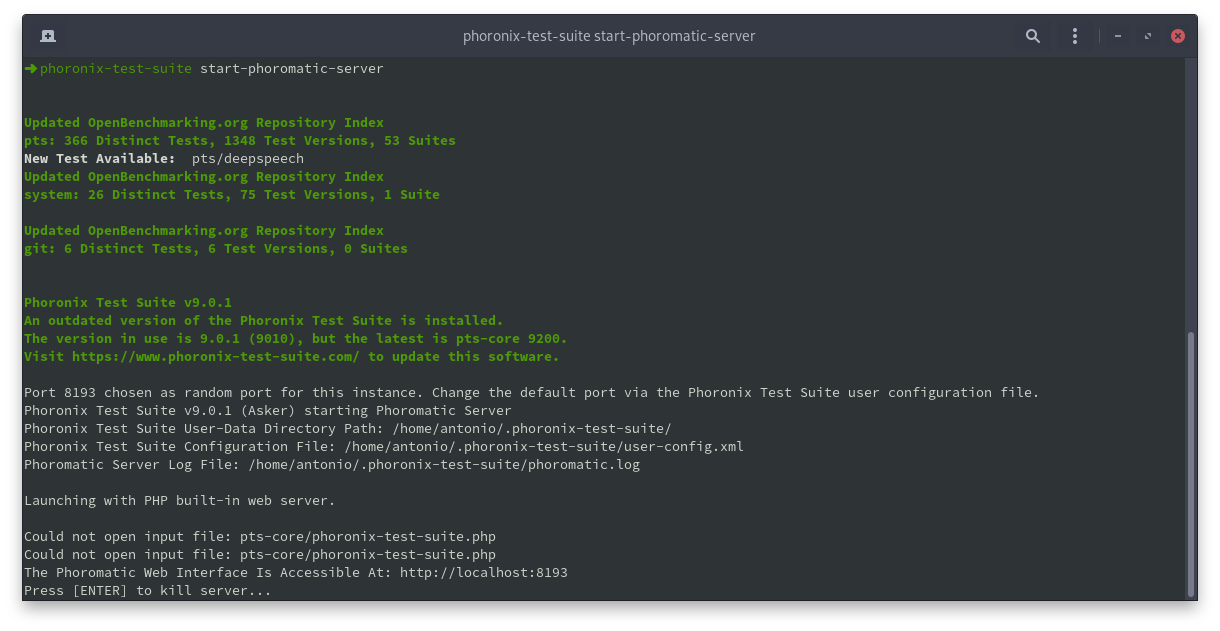
\includegraphics[scale=0.35]{phoromatic_server.png}
\end{center}


\subsection{Uso de Phoromatic}

Como podemos ver en la imagen anterior, podemos acceder a Phoromatic a través de la ruta\\ \texttt{http://localhost:8193}. Cada vez que iniciemos el servidor Phoromatic nos asignará un puerto, a no ser que especifiquemos un puerto en concreto en el archivo de configuración ubicado en\\ \texttt{$\textasciitilde$/.phoronix-test-suite/}

Al entrar en dicha URL nos pedirá un login:

\begin{center}
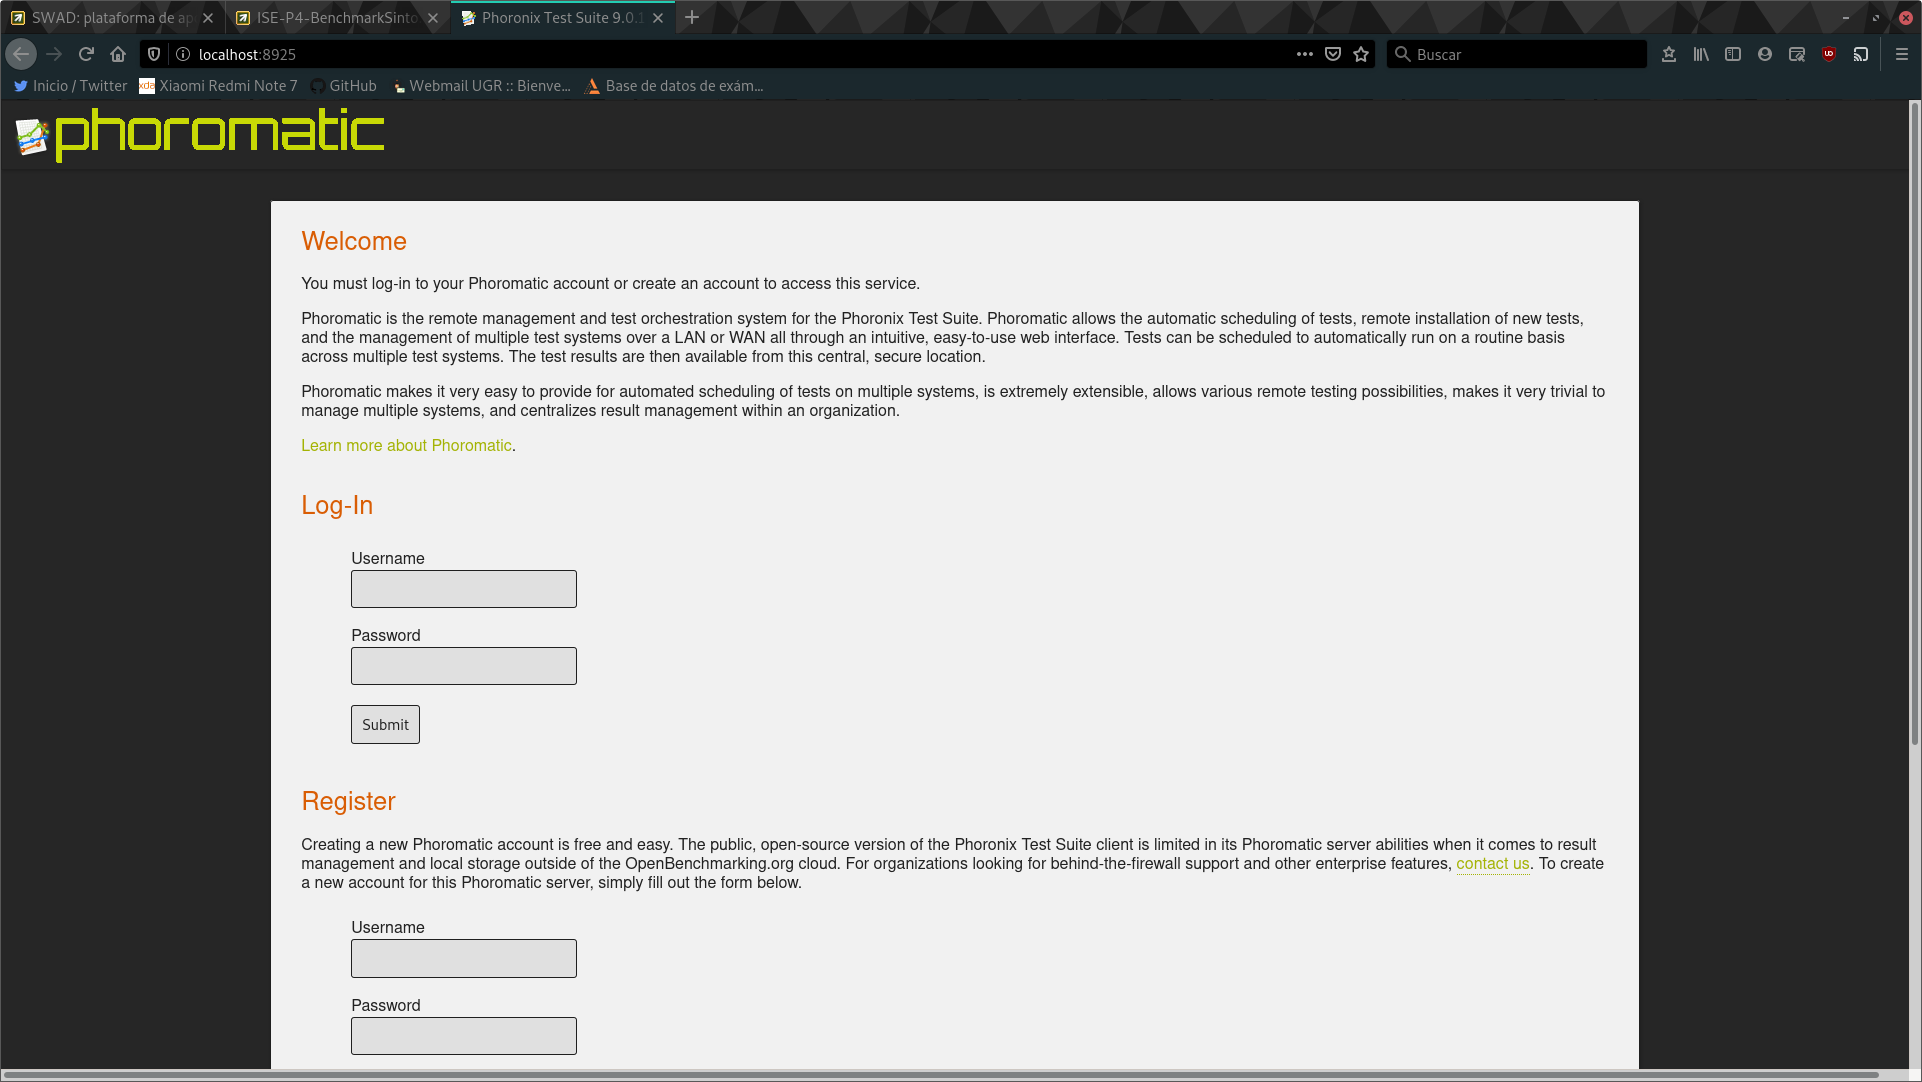
\includegraphics[scale=0.25]{login_phoromatic.png}
\end{center}

Tras registrarnos, encontraremos la siguiente página:

\begin{center}
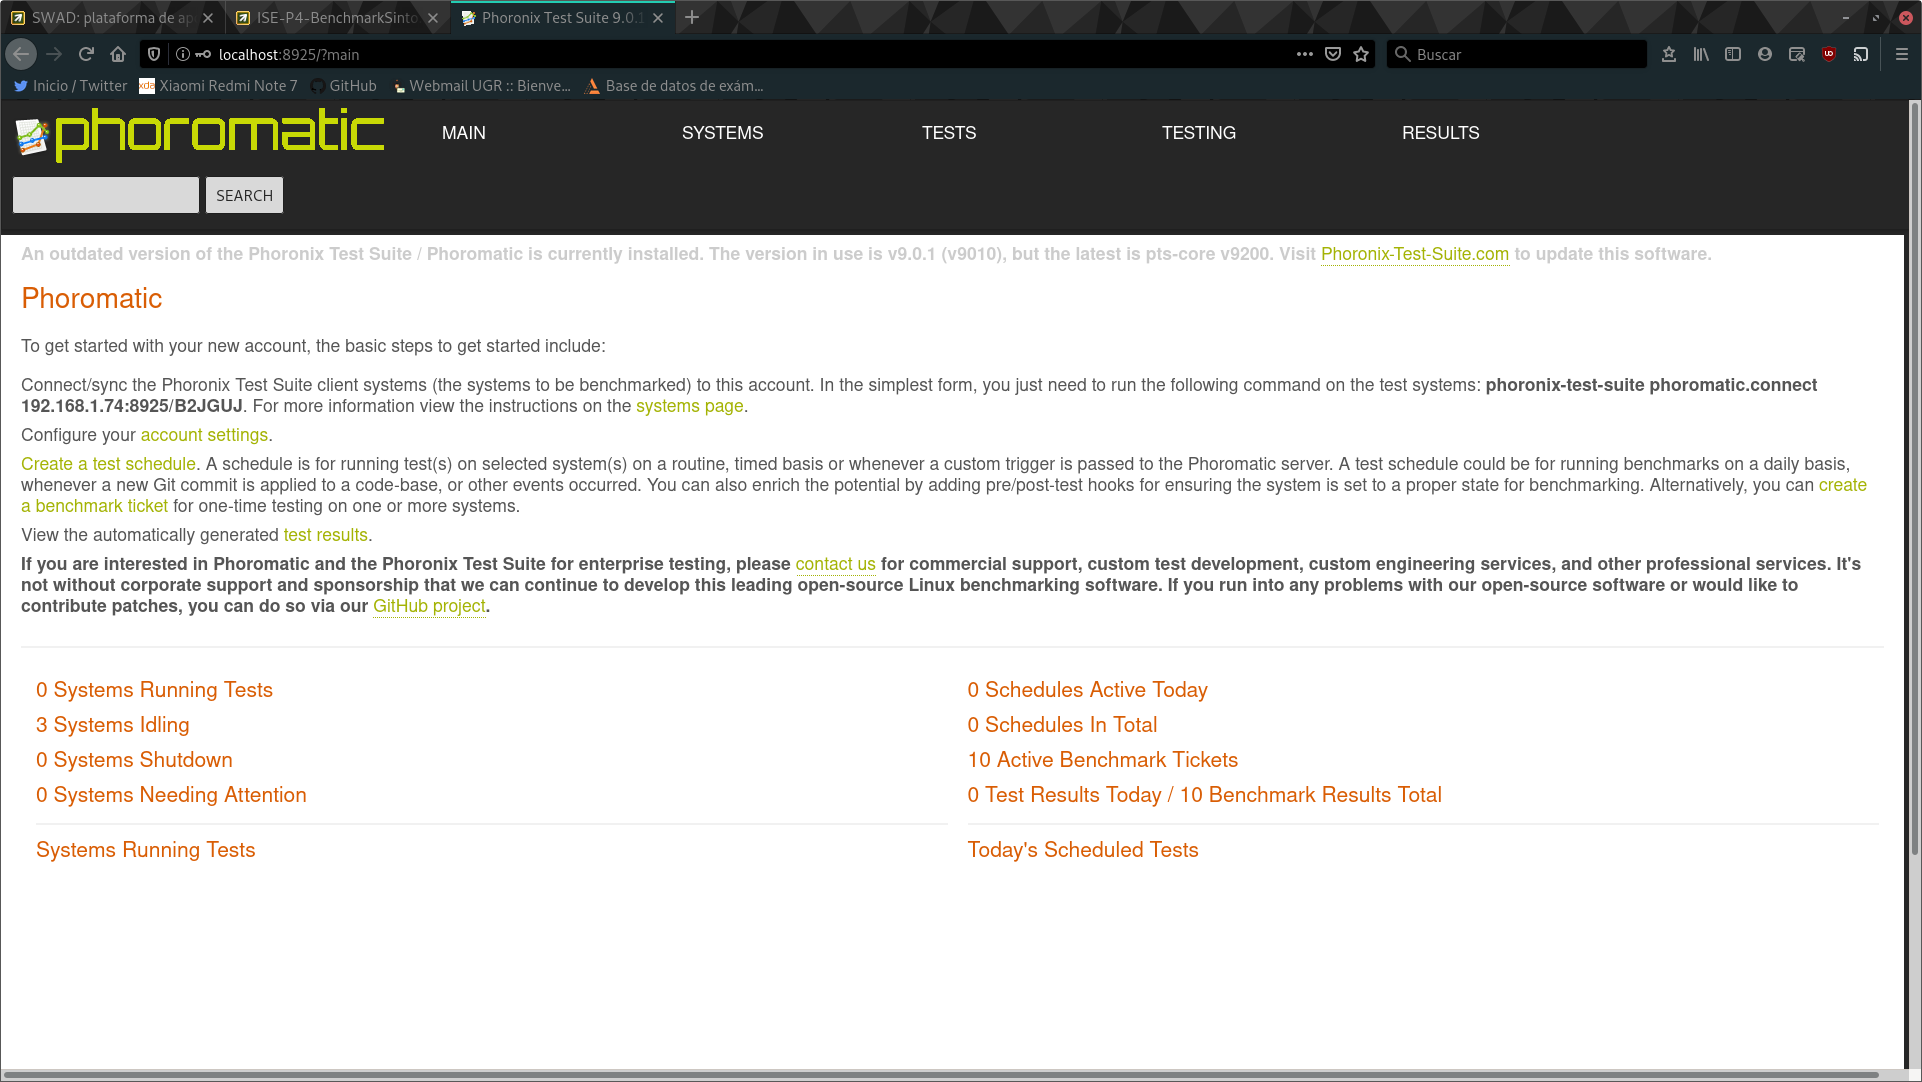
\includegraphics[scale=0.25]{main_phoromatic.png}
\end{center}

En mi caso aparecen tres máquinas, ya que tengo añadidos los tres sistemas.

\subsubsection{Añadir y conectar equipos a Phoromatic}

Como vemos en la última imagen, añadir o conectar un sistema es tan sencillo como ejecutar el comando que nos indica el servidor:

\begin{minted}[linenos,tabsize=2,breaklines]{bash}
\$ phoronix-test-suite phoromatic.connect 192.168.1.74:8925/B2JGUJ
\end{minted}

La ruta puede variar cada vez que iniciemos el servidor (a excepción de fijar una en los archivos de configuración), mientras que la última parte de la URL es un identificador único asociado al usuario de Phoromatic.

La primera vez que añadimos un equipo nos preguntará que nombre queremos asignarle dentro del servidor de Phoromatic. En mi caso los equipos se llaman CentOS-ISE, Ubuntu-ISE y antonio, siendo los dos primeros las máquinas virtuales de la asignatura y el último mi anfitrión.

En la pestaña de sistemas de Phoromatic podemos ver los sistemas que tenemos conectados, y cuando fue su ultima conexión. (La tasa de refresco es de aproximadamente uno a dos minutos.)

\begin{center}
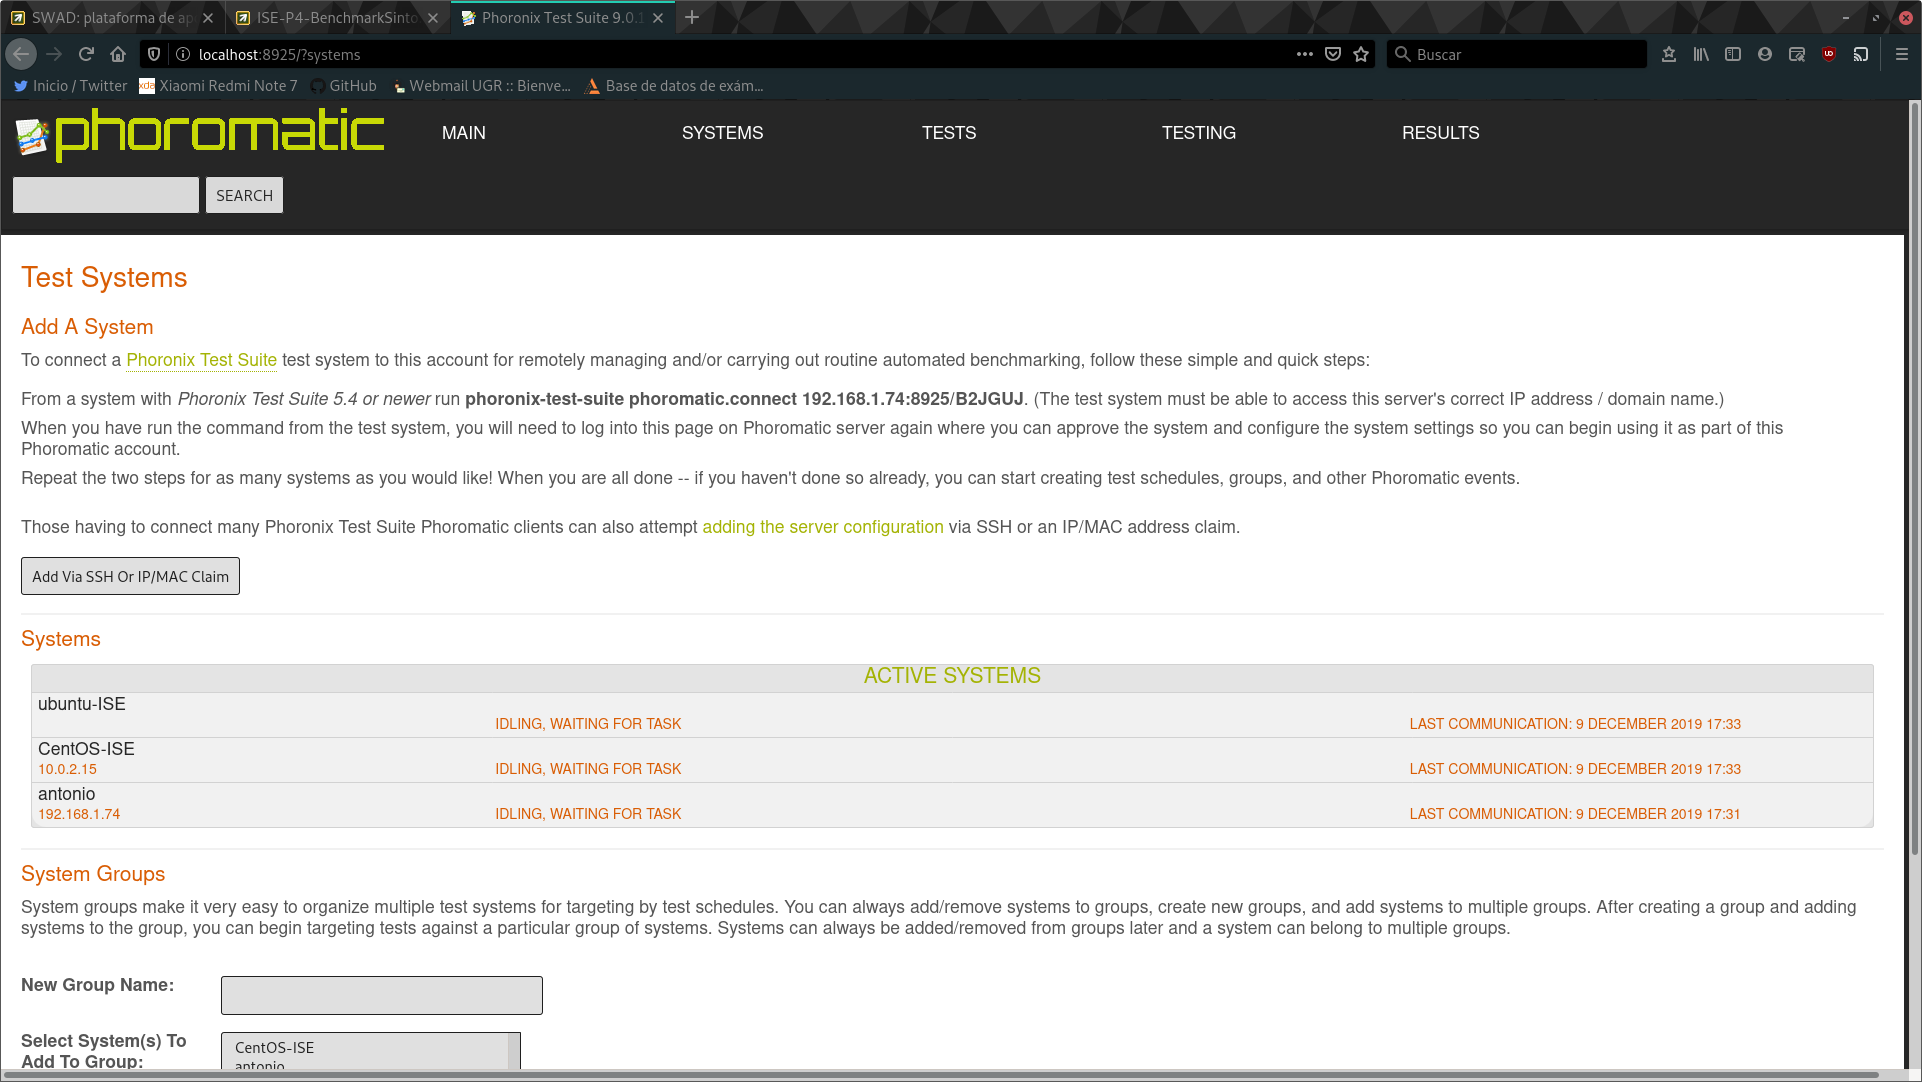
\includegraphics[scale=0.25]{phoromatic_systems.png}
\end{center}

\subsubsection{Crear Tests Suites}

En la pestaña Tests podemos crear perfiles de test, así como nuevas suites personalizadas, en nuestro caso, vamos a crear una suite que tenga como test SmallPT:

\begin{center}
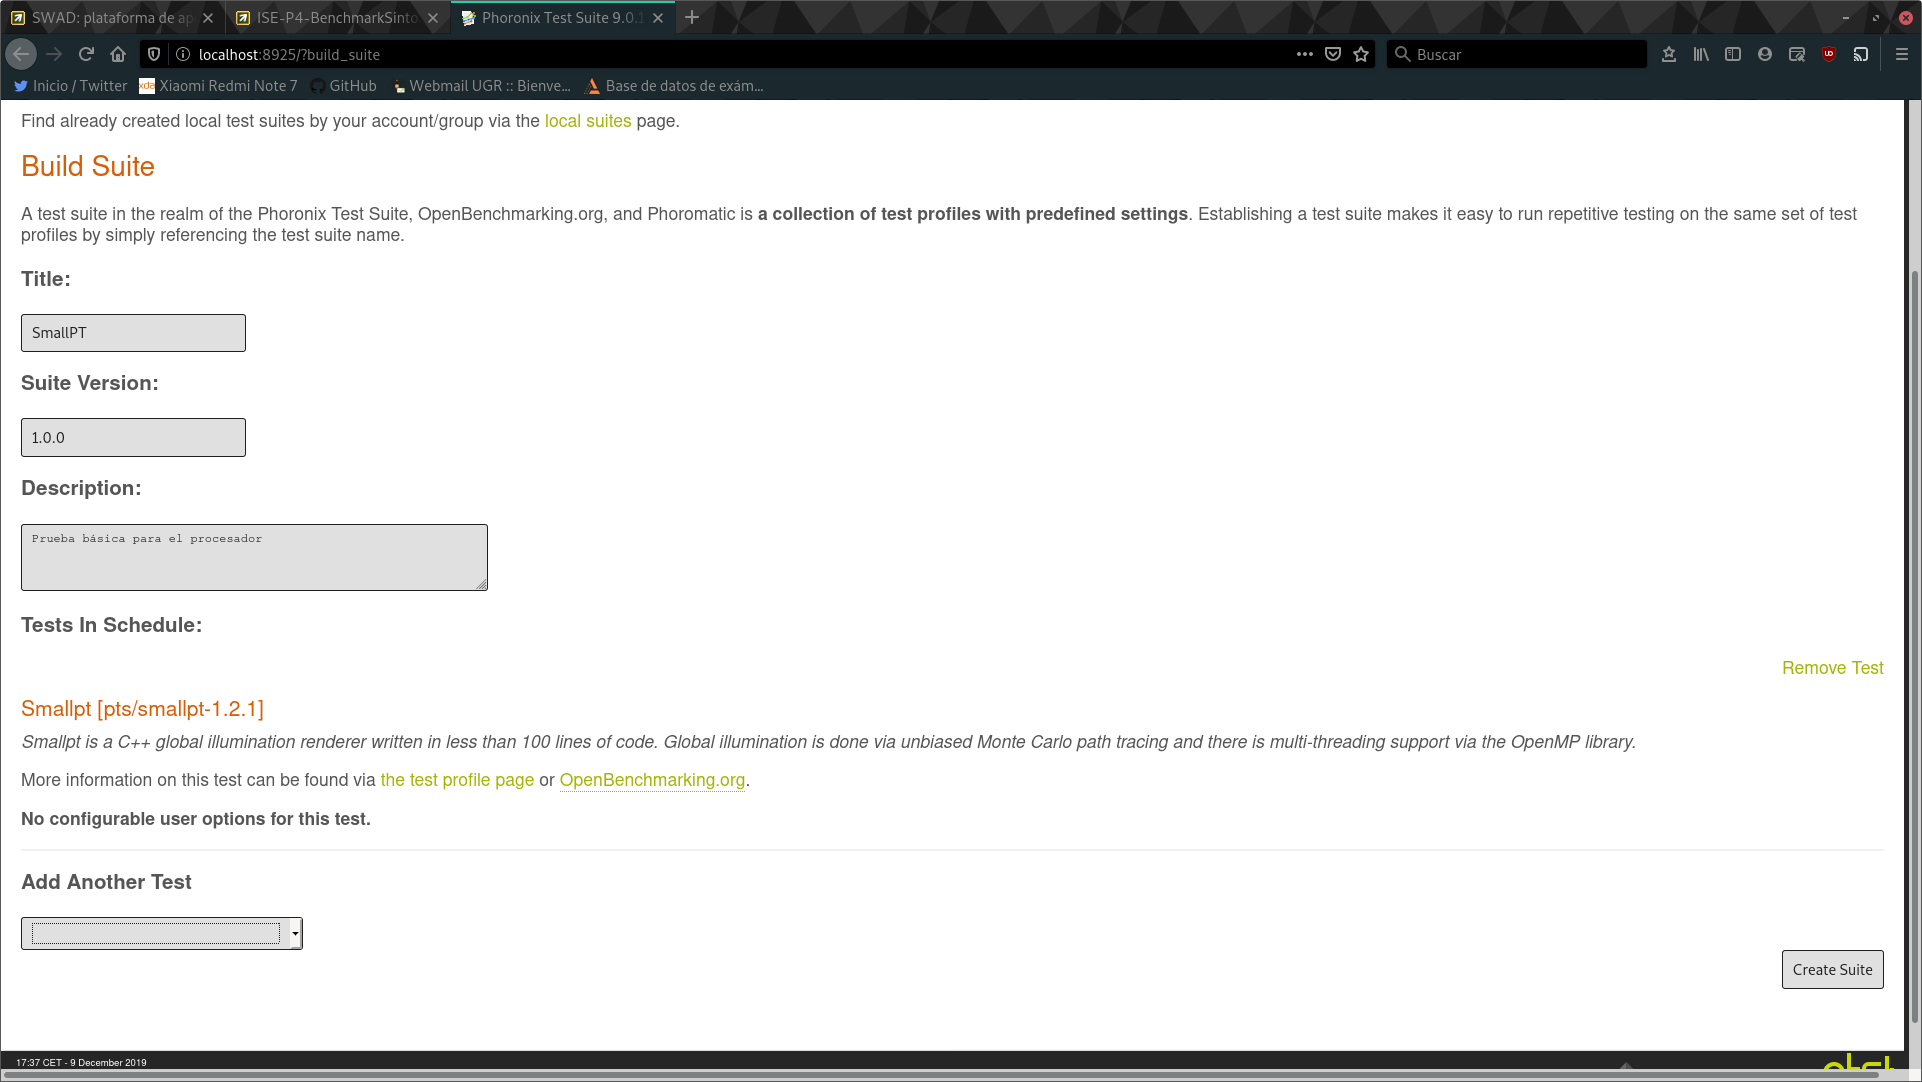
\includegraphics[scale=0.25]{phoromatic_suite.png}
\end{center}

Como vemos, podemos hacer que una suite ejecute un conjunto de tests, por si queremos, por ejemplo, aplicar distintos tests de CPU a un equipo, sin tener que ejecutarlos uno a uno manualmente.

\subsubsection{Ejecutar Suites}

En la sección Testing tenemos disponible la opción Run a benchmark, donde podemos escoger que suite ejecutar y en que sistemas ejecutarlos. En mi caso, al estar virtualizando dos de los sistemas en el anfitrión solo mandaré las pruebas a un único host simultaneamente, sin embargo, si fueran servidores distintos podríamos mandar simultaneamente suites a ejecutar.

\begin{center}
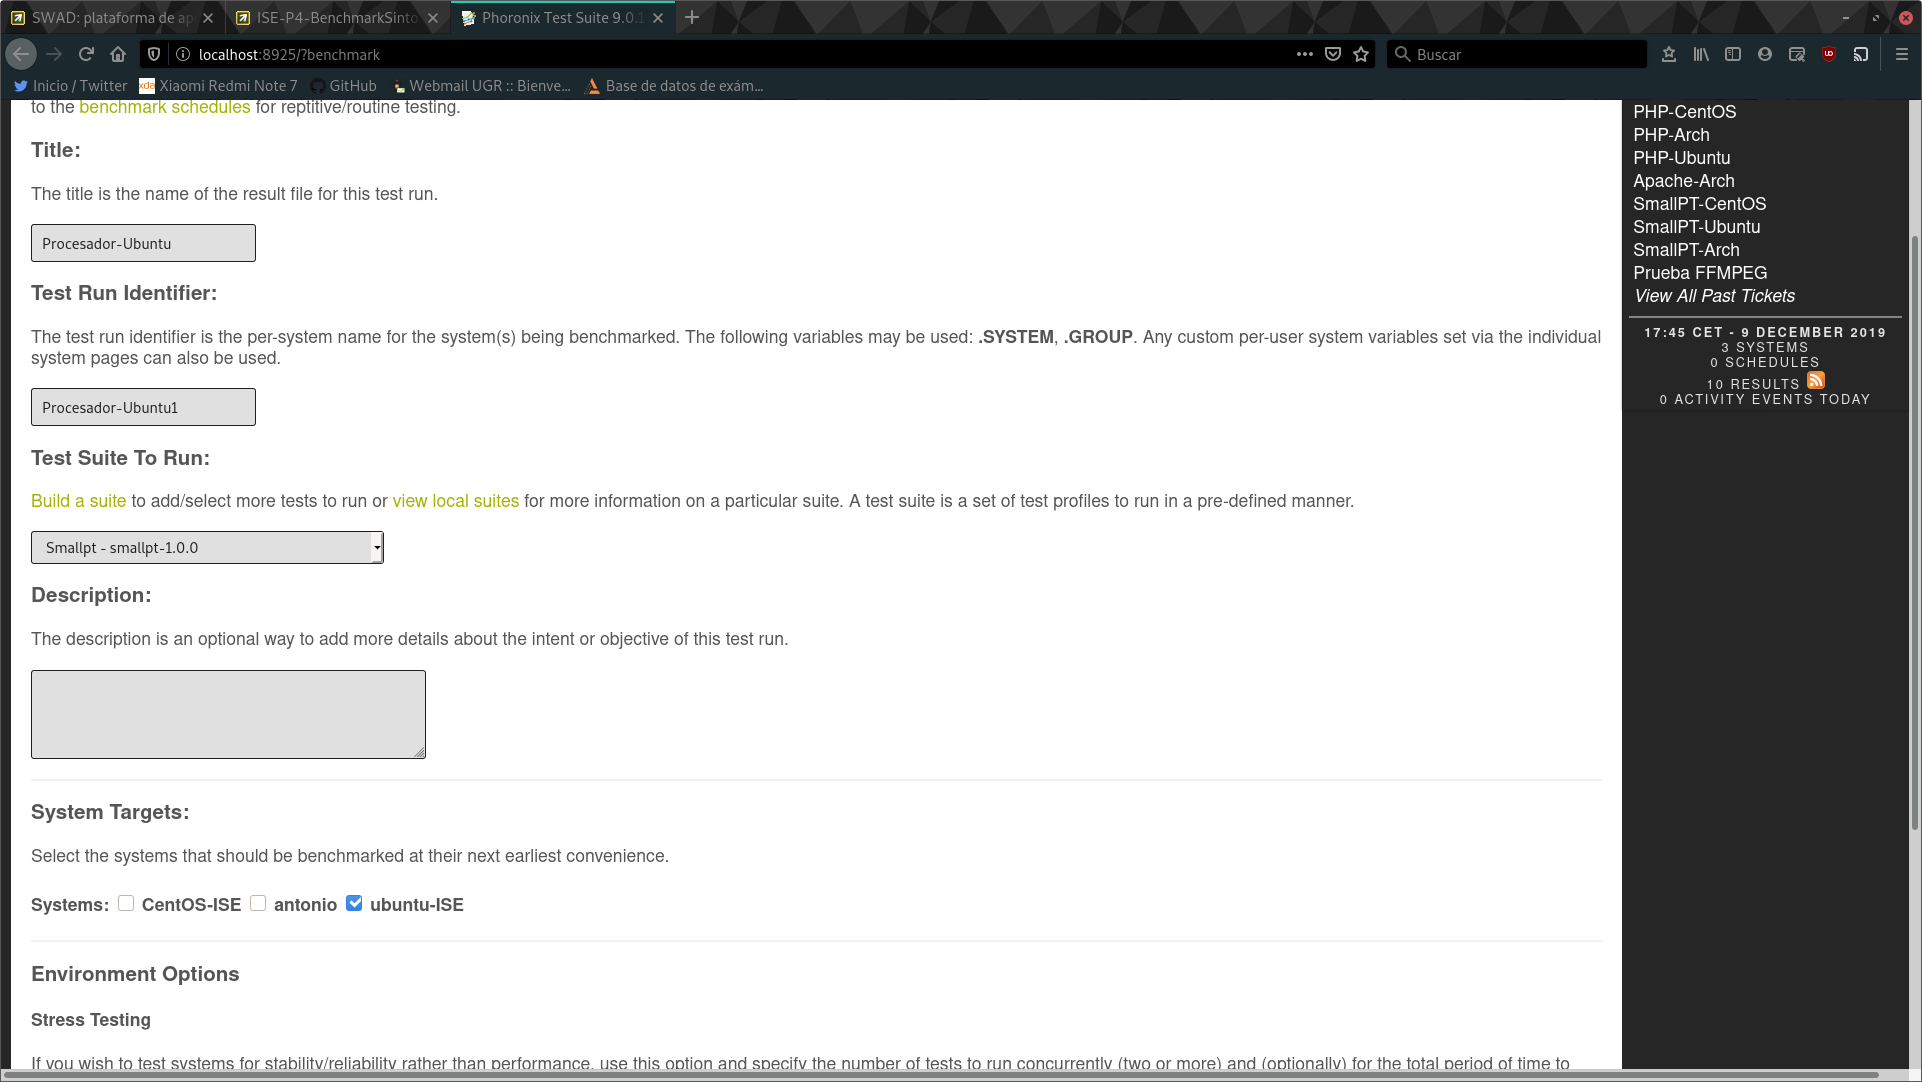
\includegraphics[scale=0.25]{phoromatic_exec.png}
\end{center}


\newpage
Vemos como también nos permite establecer el numero de concurrencia, así como el tiempo mínimo que estará ejecutando el test.

\begin{center}
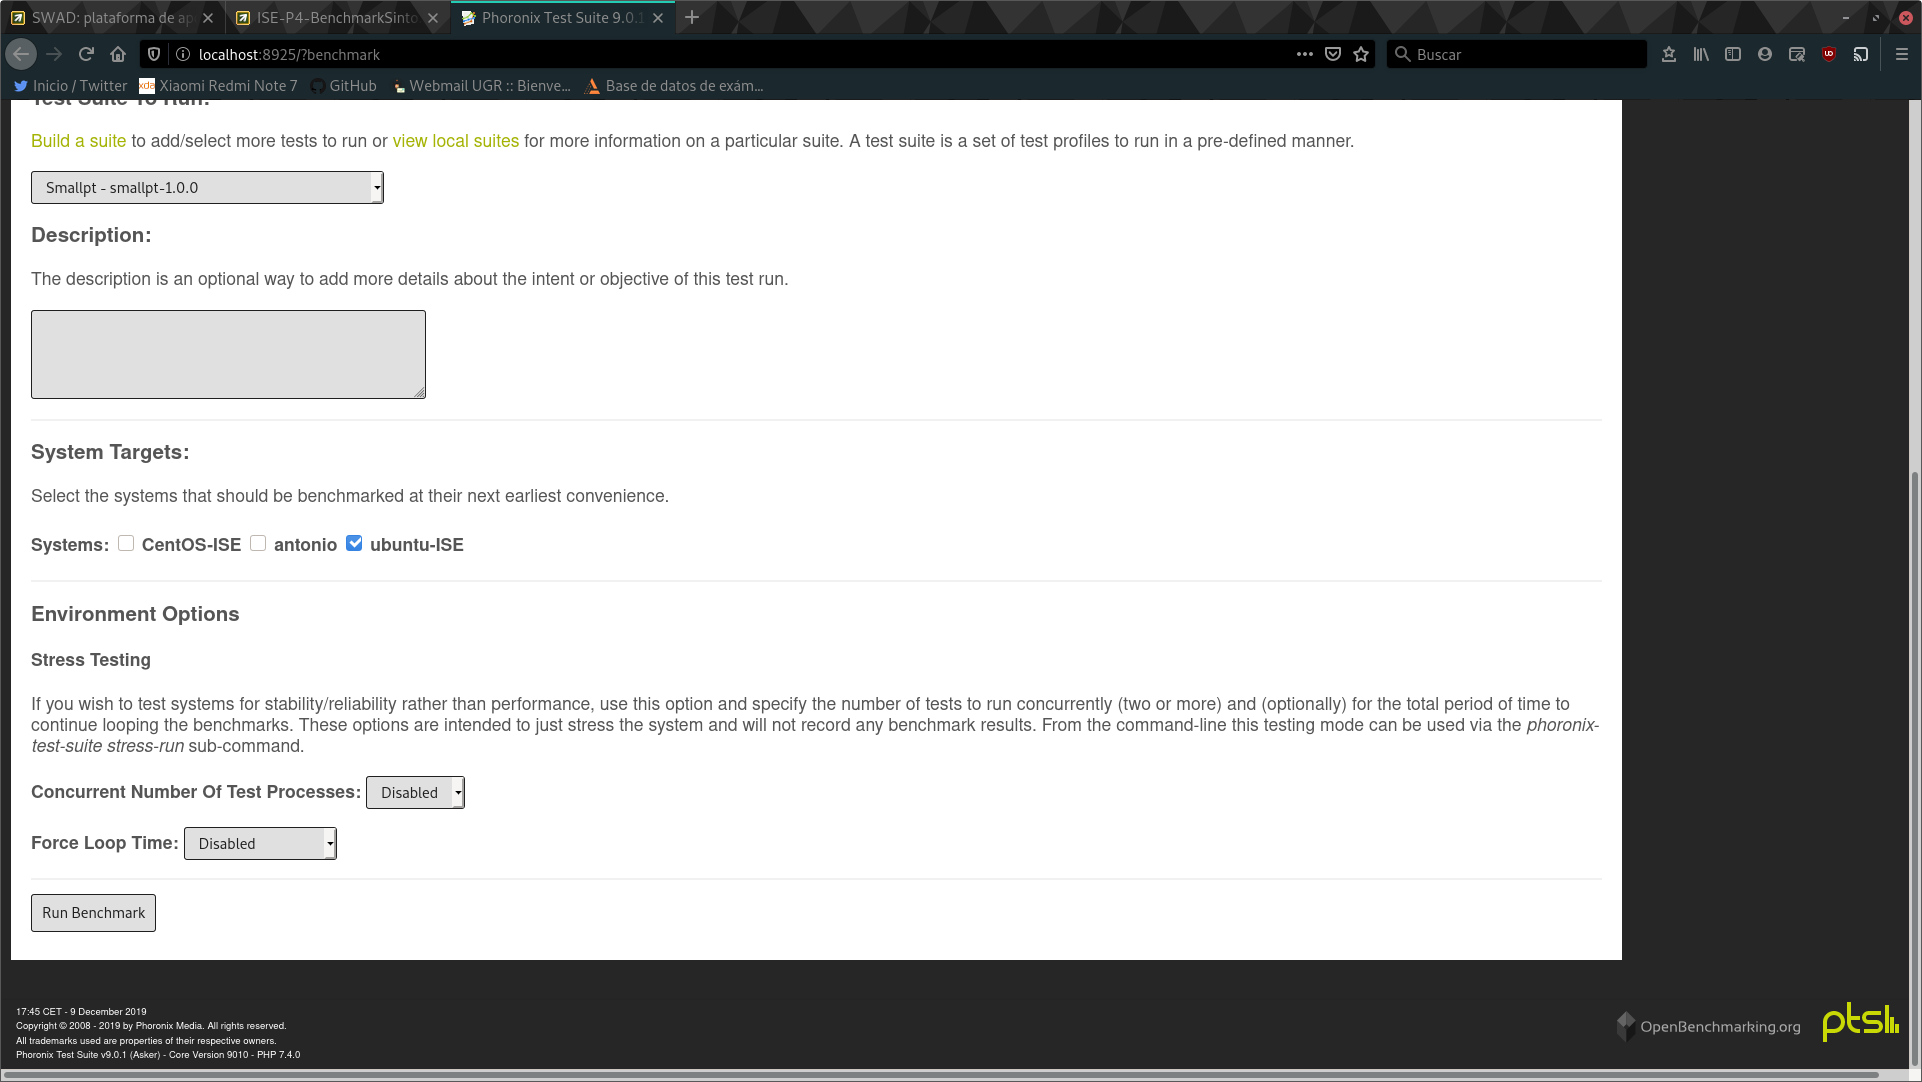
\includegraphics[scale=0.25]{phoromatic_exec2.png}
\end{center}


Una vez mandamos el benchmark, phoronix-test-suite se encargará de instalarlo, ejecutarlo, y devolver los resultados a Phoromatic.

\begin{center}
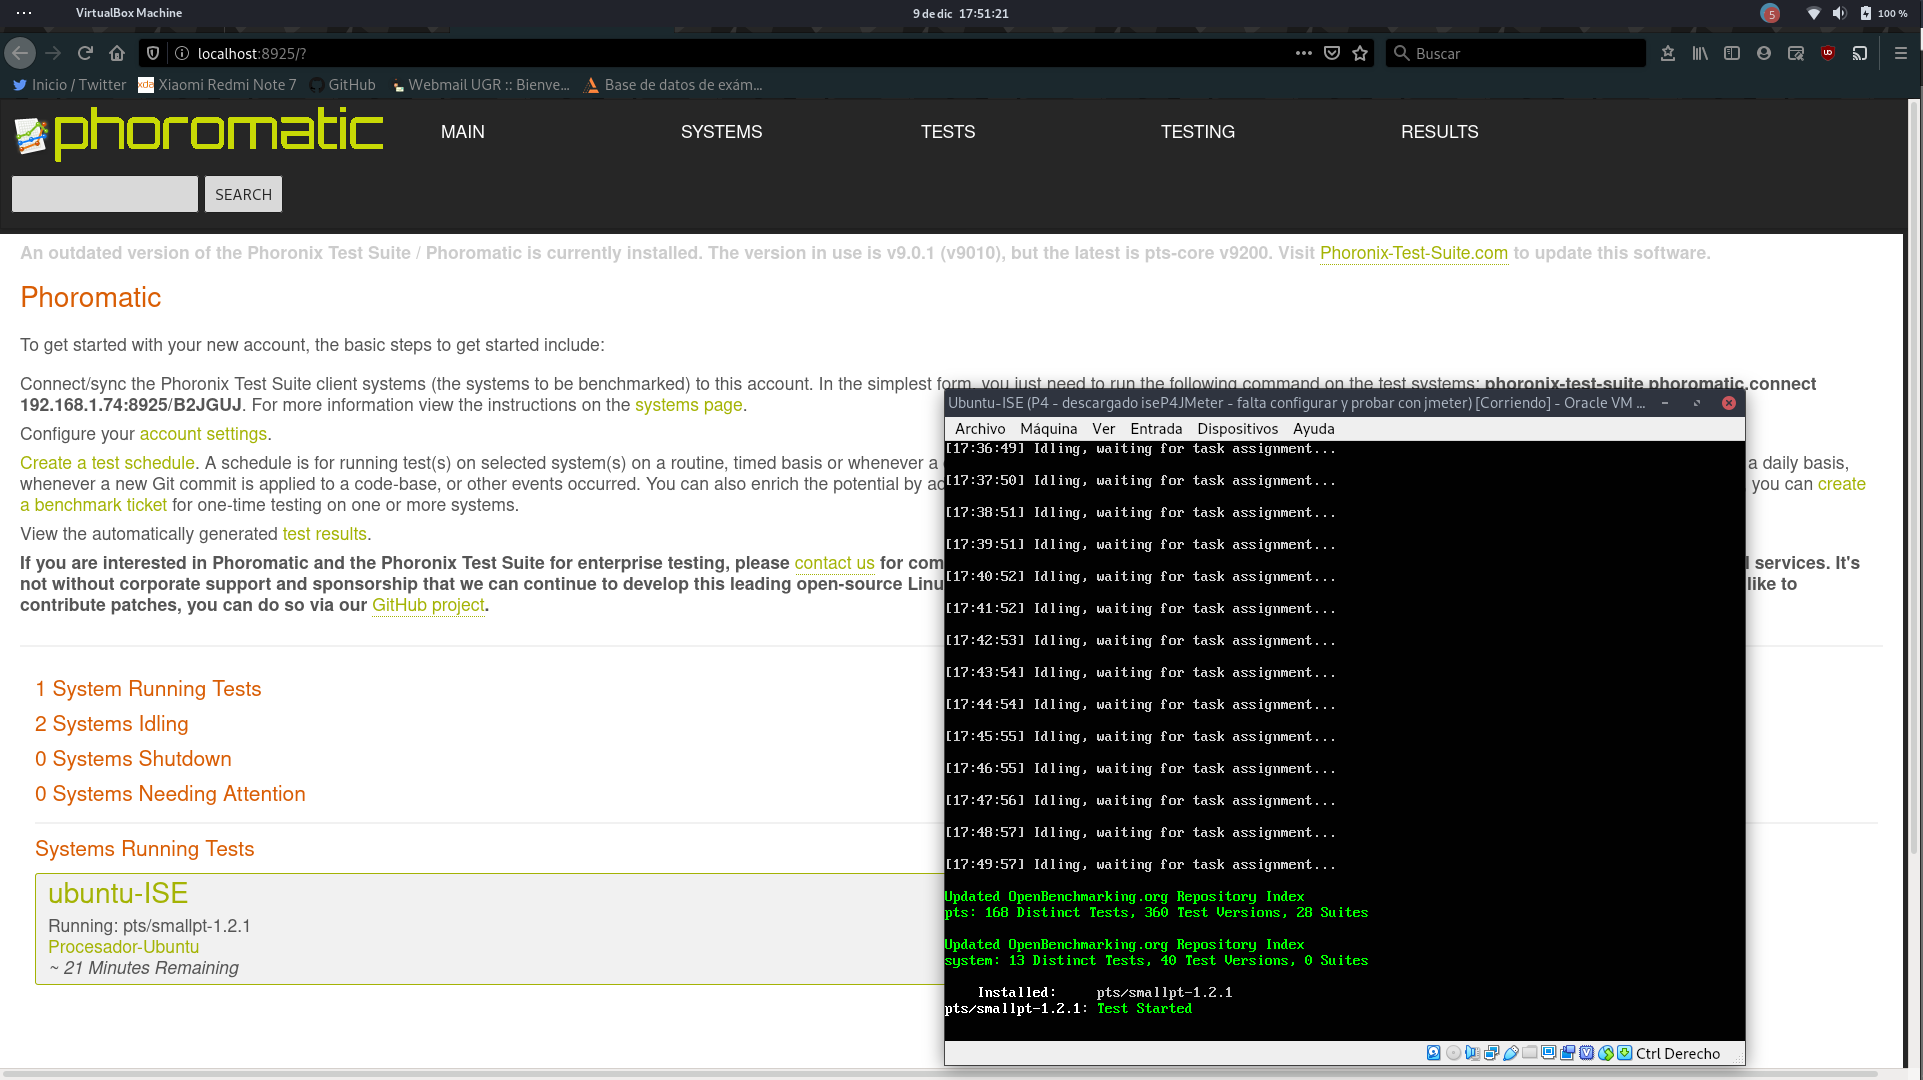
\includegraphics[scale=0.25]{phoromatic_ejecucion.png}
\end{center}


\subsubsection{Mostrar resultados}

En la opción de Results tenemos disponibles los distintos resultados:

\begin{center}
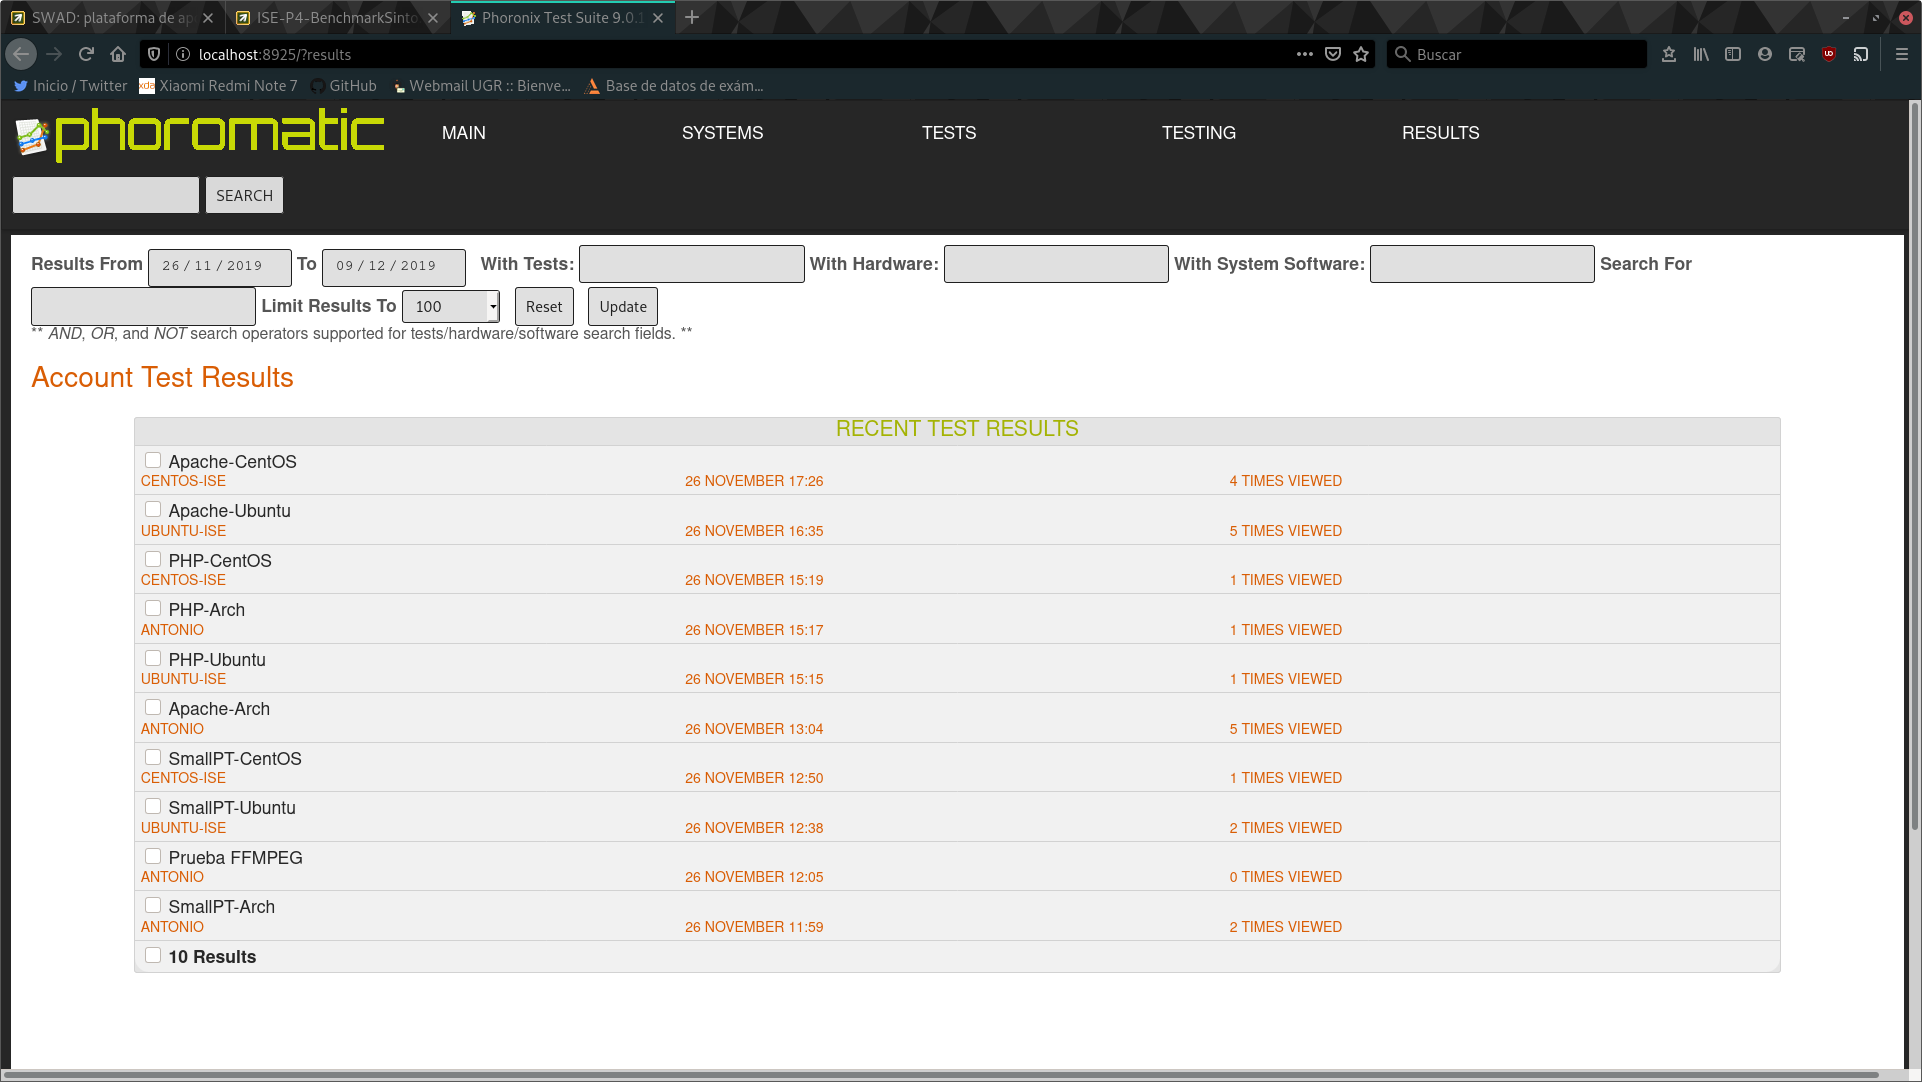
\includegraphics[scale=0.25]{phoromatic_results.png}
\end{center}

Podemos escoger varios (o solo uno) y compar los resultados, pinchando en la nueva opción del menú: Compare


\begin{center}
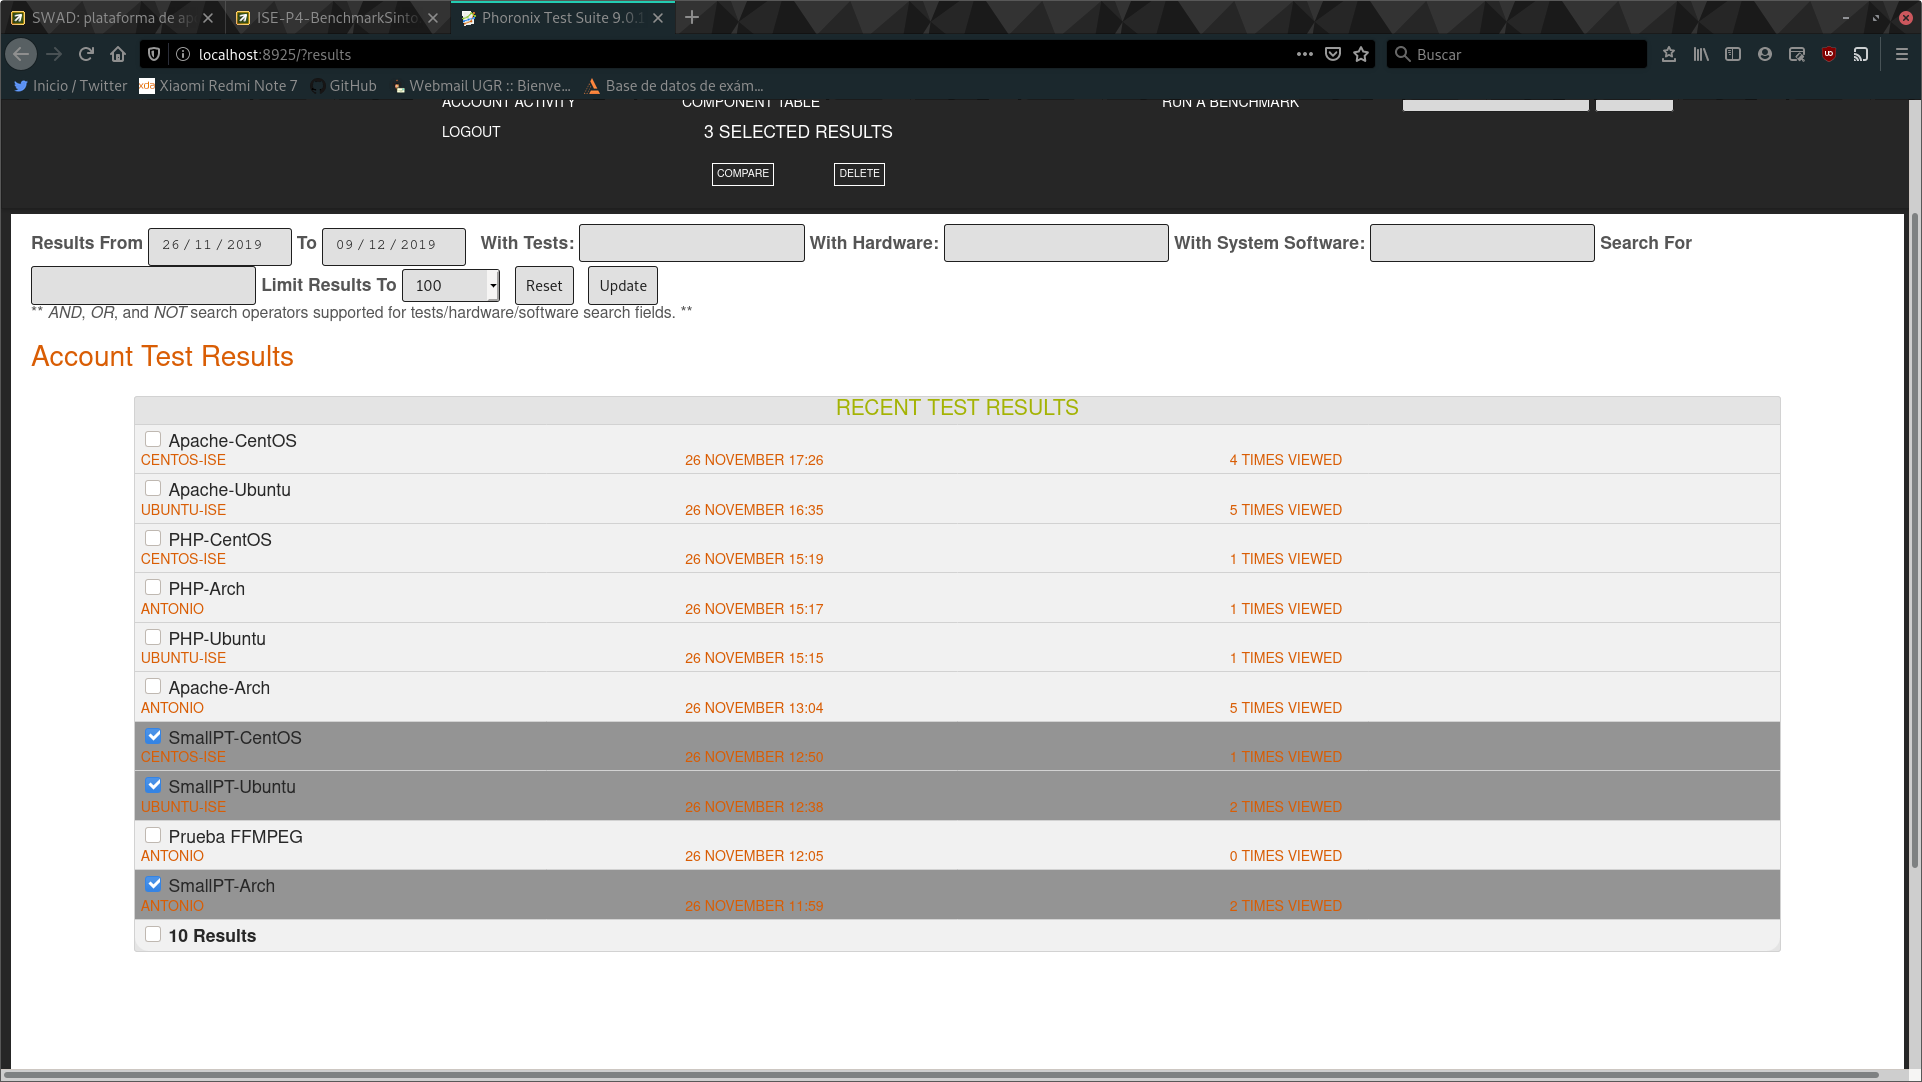
\includegraphics[scale=0.25]{phoromatic_compare.png}
\end{center}

Nos aparecerá esta pestaña, donde tenemos información de cada sistema, así como los resultados:

\begin{center}
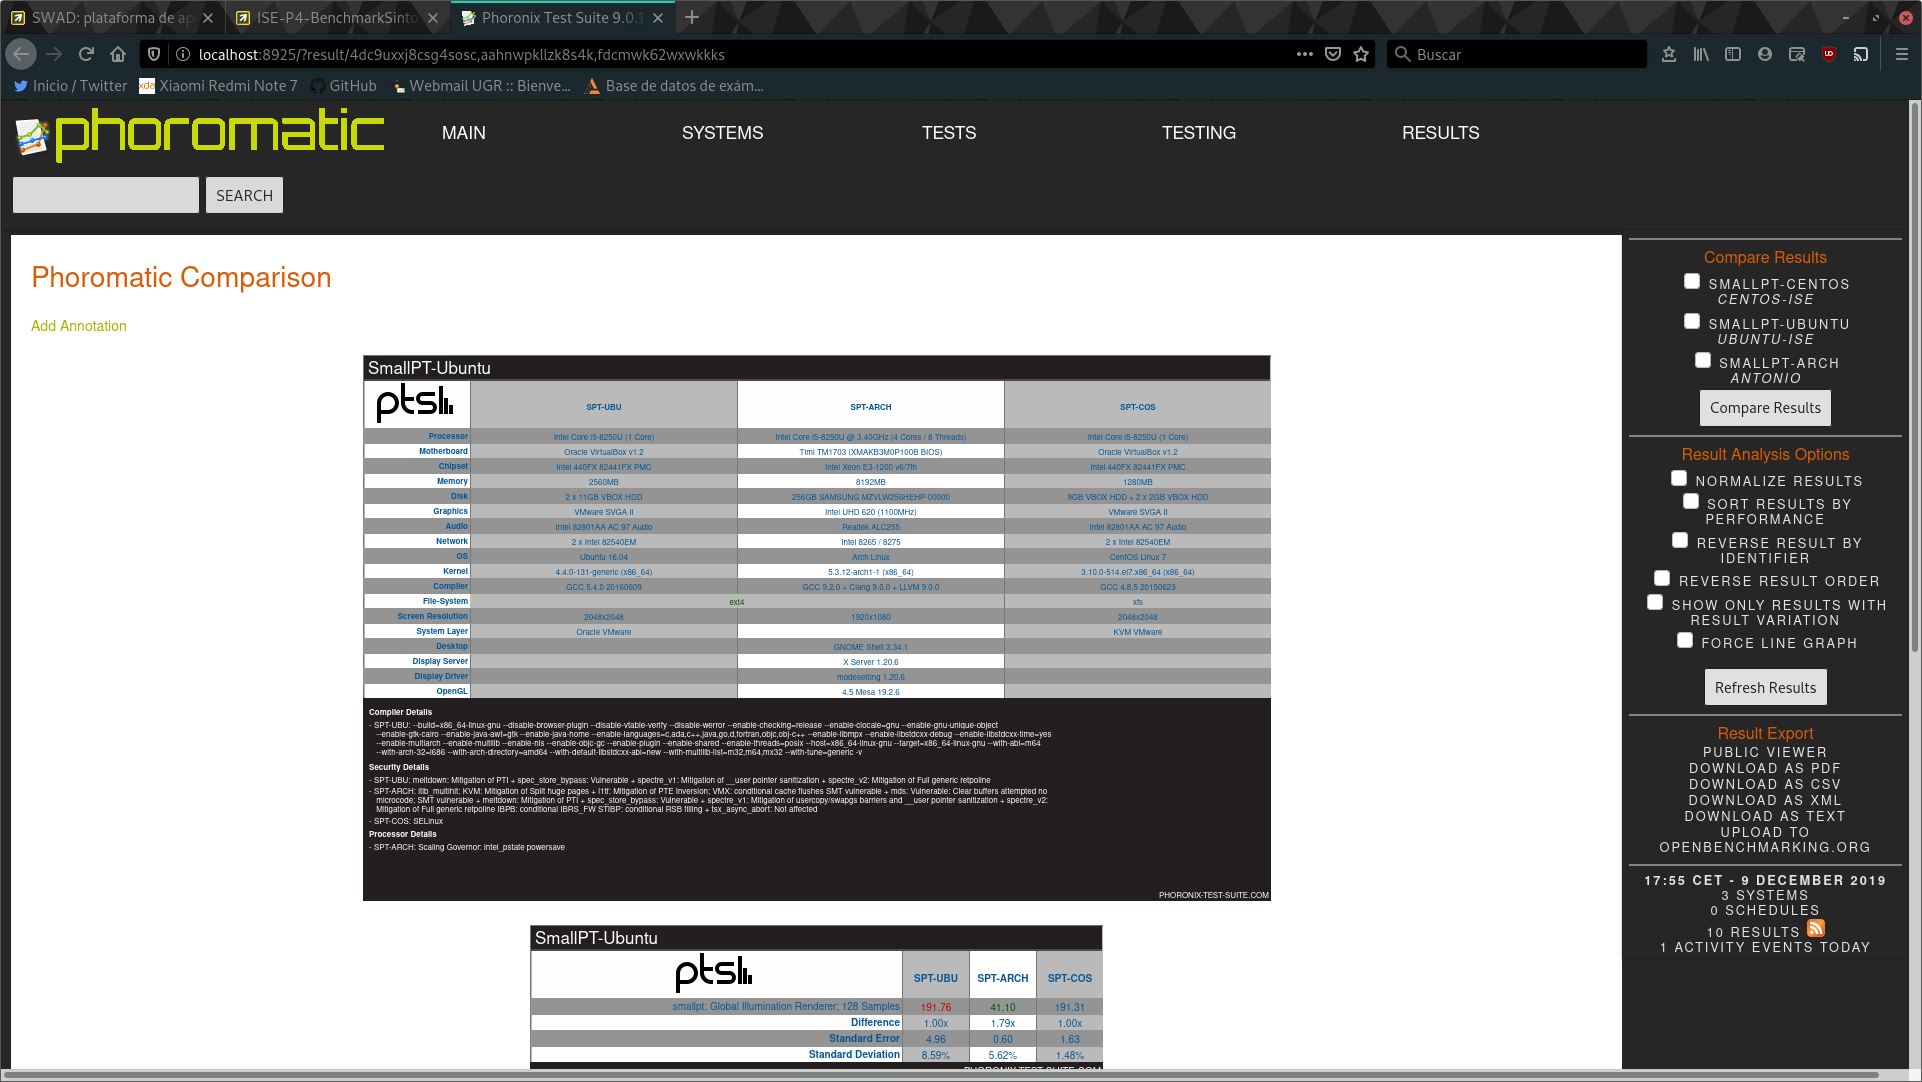
\includegraphics[scale=0.25]{phoromatic_datos.png}
\end{center}

\begin{center}
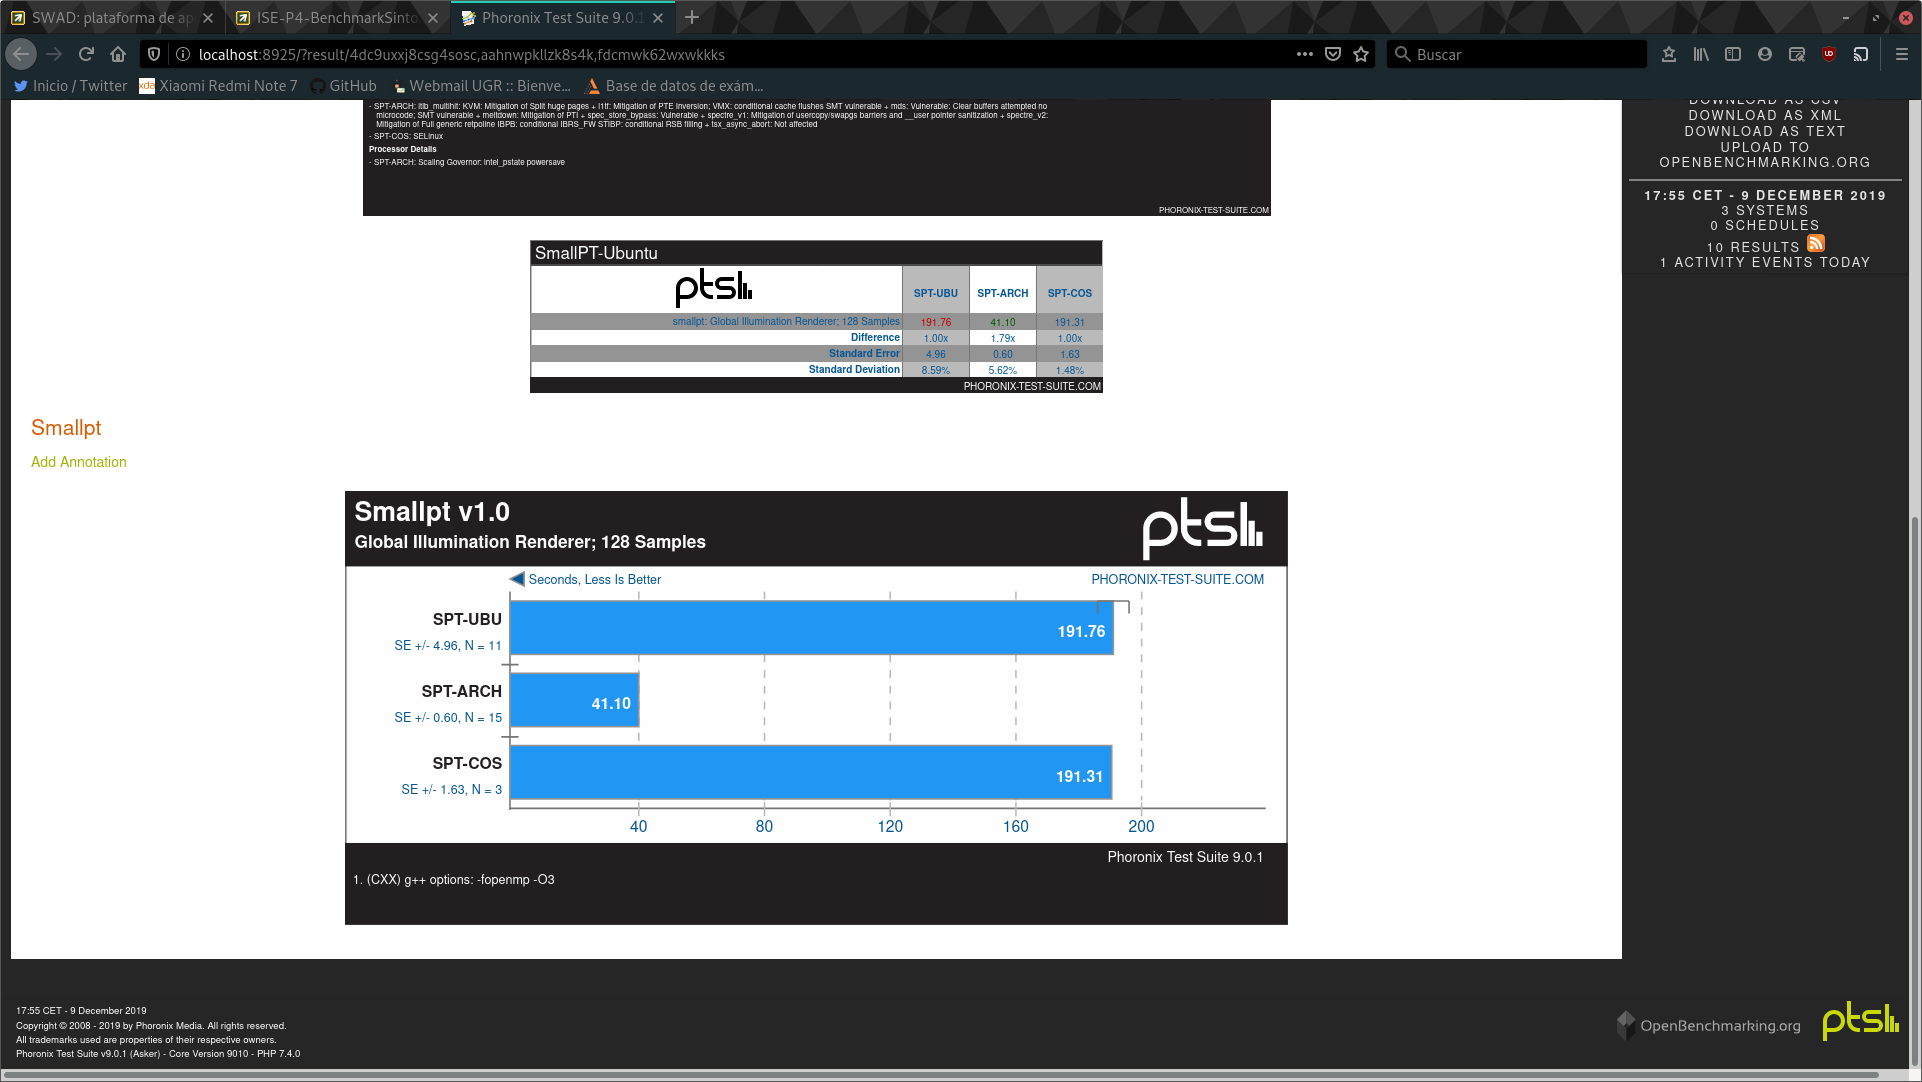
\includegraphics[scale=0.25]{phoromatic_graph.png}
\end{center}

%\section{Apache AB}

%\subsection{Instalación de Apache AB}

%\section{JMeter}

%\subsection{Instalación de JMeter}



\newpage

\begin{thebibliography}{9}

\bibitem{pts}
Phoronix Test Suite \url{https://www.phoronix-test-suite.com/}

\bibitem{obm}
OpenBenchmarking \url{https://www.openbenchmarking.org/}

\bibitem{yay}
Yet Another Yogurt \url{https://github.com/Jguer/yay}

\bibitem{pts_descarga}
Phoronix Test Suite - Descarga \url{https://www.phoronix-test-suite.com/?k=downloads}

\bibitem{pts_docker}
Docker Phoronix Test Suite \url{https://hub.docker.com/r/phoronix/pts/}

\bibitem{pts_man}
Man phoronix-test-suite \url{https://linux.die.net/man/1/phoronix-test-suite}

\end{thebibliography}


\end{document}
